%%%%%%%%%%%%%%%%%%%%%%%%%%%%%%%%%%%%%%%%%%%%%%%%%%%%%%%%%%%%%%%%%%%%%%%%%%%

\documentclass{standalone}

\usepackage{amsmath}
\usepackage{mathptmx}
\usepackage{pgfplots}
\usetikzlibrary{external}
\tikzexternalize{radioactive-dice}
\pgfplotsset{compat=1.16}

%% IEEE uses Times Roman font, so we'll default to Times.
%% These three commands make up the entire times.sty package.
\renewcommand{\rmdefault}{ptm}
\renewcommand{\ttdefault}{pcr}
\normalfont\selectfont

\begin{document}

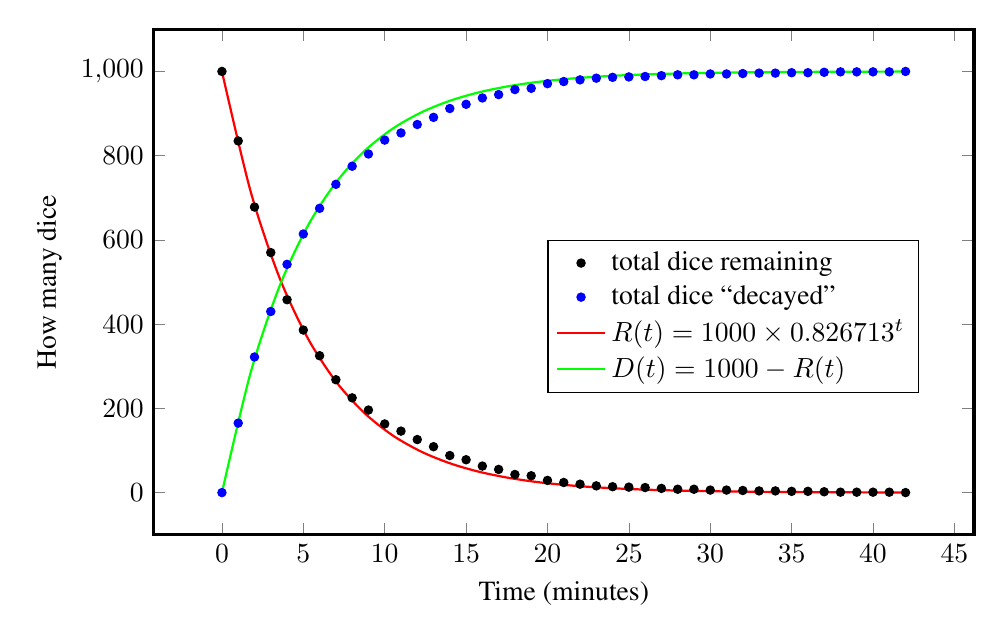
\begin{tikzpicture}
\tikzset{%%
  every mark/.append style={scale=1.0},%%
  scale=1.0%%
}
\pgfplotsset{%%
  every axis/.append style={font=\normalsize}%%
}
%%
\begin{axis}[%%
  axis line style=very thick,%%
  dotStyle/.style={mark size=1.5,mark=*,only marks},%%
  enlargelimits=true,%%
  height=8cm,%%
  legend cell align=left,%%
  legend style={at={(axis cs:20,600)},anchor=north west},%%
  plotStyle/.style={%%
    domain=0:42,%%
    mark=none,%%
    smooth,%%
    thick%%
  },%%
  width=12cm,%%
  %% x axis
  xlabel={\normalsize Time~(minutes)},%%
  %% y axis
  ylabel={\normalsize How many dice},%%
  scaled y ticks=false,%%
  y tick label style=/pgf/number format/fixed%%
]
%%
%%
%% How many "undecayed" dice.
\addplot[dotStyle,black] coordinates {
  (0, 1000)
  (1, 835)
  (2, 678)
  (3, 570)
  (4, 458)
  (5, 386)
  (6, 325)
  (7, 268)
  (8, 225)
  (9, 196)
  (10, 163)
  (11, 146)
  (12, 126)
  (13, 109)
  (14, 88)
  (15, 78)
  (16, 63)
  (17, 55)
  (18, 43)
  (19, 40)
  (20, 29)
  (21, 24)
  (22, 20)
  (23, 16)
  (24, 14)
  (25, 13)
  (26, 12)
  (27, 10)
  (28, 8)
  (29, 8)
  (30, 6)
  (31, 6)
  (32, 5)
  (33, 4)
  (34, 4)
  (35, 3)
  (36, 3)
  (37, 2)
  (38, 1)
  (39, 1)
  (40, 1)
  (41, 1)
  (42, 0)
};
\addlegendentry{total dice remaining}
%%
%%
%% Cumulative sum of "decayed" dice.
\addplot[dotStyle,blue] coordinates {
  (0, 0)
  (1, 165)
  (2, 322)
  (3, 430)
  (4, 542)
  (5, 614)
  (6, 675)
  (7, 732)
  (8, 775)
  (9, 804)
  (10, 837)
  (11, 854)
  (12, 874)
  (13, 891)
  (14, 912)
  (15, 922)
  (16, 937)
  (17, 945)
  (18, 957)
  (19, 960)
  (20, 971)
  (21, 976)
  (22, 980)
  (23, 984)
  (24, 986)
  (25, 987)
  (26, 988)
  (27, 990)
  (28, 992)
  (29, 992)
  (30, 994)
  (31, 994)
  (32, 995)
  (33, 996)
  (34, 996)
  (35, 997)
  (36, 997)
  (37, 998)
  (38, 999)
  (39, 999)
  (40, 999)
  (41, 999)
  (42, 1000)
};
\addlegendentry{total dice ``decayed''}
%%
%%
%% The number R(t) of dice remaining after t minutes.  The prediction
%% function was obtained by estimating the decay constant.
\addplot+ [plotStyle,red]
{1000 * (0.826713^x)};
\addlegendentry{$R(t) = 1000 \times 0.826713^t$}
%%
%%
%% The total number D(t) of dice that have "decayed" after t minutes.
%% The prediction function was derived as D(t) = 1000 - R(t).
\addplot+ [plotStyle,green]
{1000 * (1 - 0.826713^x)};
\addlegendentry{$D(t) = 1000 - R(t)$}
\end{axis}
\end{tikzpicture}

\end{document}
